\documentclass{article}

\usepackage{spconf}
\usepackage{amsmath,graphicx}
\usepackage{color}
\usepackage{url}

\usepackage{fancyhdr}
\usepackage{lipsum}

\def\x{{\mathbf x}}
\def\L{{\cal L}}

\title{An Experimental Study on Audio Replay Attack Detection Using Deep Neural Networks}

\name{Bekir Bakar, Cemal Hanil\c{c}i\thanks{This work was supported by the Scientific and Technological Research
Council of Turkey (T\"{U}B\.{I}TAK) (project no. 115E916) .}}
\address{ Bursa Technical University\\
Department of Electrical and Electronics Engineering\\
Bursa, Turkey}

\fancypagestyle{aps}{\fancyhf{}\renewcommand{\headrulewidth}{0pt}
\fancyfoot[C]{\thepage{}}}
\pagestyle{aps}
\setcounter{page}{132}

\fancypagestyle{sps}{\fancyhf{}\renewcommand{\headrulewidth}{0pt}
\fancyfoot[L]{978-1-5386-4334-1/18/\$31.00 \copyright\ 2018 IEEE\hfill}
\fancyfoot[R]{SLT 2018}
\fancyfoot[C]{\thepage{}}}
\thispagestyle{sps}

\begin{document}

\maketitle

\begin{abstract}
    \label{abstract}
    Automatic speaker verification (ASV) systems can be easily spoofed by previously recorded speech, synthesized
    speech and speech signal that artificially generated by voice conversion techniques. In order to increase the
    reliability of the ASV systems, detecting spoofing attacks whether a given speech signal is genuine or spoofed
    plays an important role. In this paper, we consider the detection of replay attacks which is the most accessible
    attack type against ASV systems. To this end, we utilize a deep neural network (DNN) based classifier using
    features extracted from the long-term average spectrum. The experiments are conducted on the latest edition of
    Automatic Speaker Verification Spoofing and Countermeasures Challenge (ASVspoof 2017) database. The results are
    compared with the ASVspoof 2017 baseline system which consists of Gaussian mixture model (GMM) classifier with
    constant-Q transform cepstral coefficients (CQCC) front-end as well as the GMM with standard mel-frequency cepstrum
    coefficients (MFCC) features. Experimental results reveal that DNN considerably outperforms the well-known and
    successful GMM classifier. It is found that long term average spectrum (LTAS) based features are superior to CQCC
    and MFCC in terms of equal error rate (EER). Finally, we find that high-frequency components convey much more
    discriminative information for replay attack detection independent of features and classifiers.
\end{abstract}

\begin{keywords}
    speaker verification, replay attack detection, deep neural networks, countermeasures
\end{keywords}

\section{Introduction}
\label{sec:intro}
% Speaker Recognition Definition
Automatic speaker verification (ASV) is the task of verifying the identity of an individual using his/her speech
signal \cite{kinnunen2010overview}. Two kinds of errors can occur in any ASV system: (i) rejecting a valid identity
claim, namely, false rejection and (ii) accepting an impostor identity claim which is known as false acceptance or
false alarm. Although, ASV systems are desired to be error-free, there is a trade-off between these two types of error
and it depends on the type of application in practice.

% Problem Definition
ASV systems are widely used in many cases that require user authentication such as call centers, telephone banking,
and forensic applications. Therefore, the reliability of these systems plays an important role. Unfortunately, similar
to other popular biometric recognition tools (e.g. face and fingerprint recognition) ASV systems were found to be
highly vulnerable against spoofing attacks which eventually increase the false acceptance rates (FAR) considerably
\cite{alegre2014re, hadid2015biometrics, ergunay2015vulnerability, wu2016study,villalba2010speaker}. Although
state-of-the-art techniques yield high speaker recognition accuracy, it was shown that their performance drastically
decrease in case of sensor-level attack (also known as presentation attack or spoofing attack) \cite{wu2015sas,
    wu2015spoofing}.

% ASVspoof Competition and Fundamental Observations
ASV systems can directly be spoofed by voice mimicry \cite{hautamaki2015automatic}, speech synthesis (SS)
\cite{de2012evaluation}, voice conversion (VC) \cite{stylianou2009voice} and replay attacks \cite{alegre2014re}.
Therefore detecting the spoofing attacks has become a hot topic for the ASV community. To this end, Automatic Speaker
Verification Spoofing and Countermeasures Challenge (ASVspoof 2015) was organized in 2015 \cite{wu2015asvspoof}. The
aim of this first competition was to develop countermeasures against SS and VC attacks on a standard database. Later,
the ASVspoof challenge was organized in 2017 again and it was mainly focused on detecting the replay attacks rather
than SS and VC attacks \cite{kinnunen2017asvspoof}. As a result of ASVspoof 2015 and 2017 challenges, many
countermeasures have been proposed for spoofing attack detection \cite{sahidullah2015comparison, li2017study,
    witkowski2017audio}. For example, it was found that the high-frequency region conveys more discriminative
information for detecting SS and VC attacks for magnitude spectrum based features \cite{sahidullah2015comparison}.
Phase features (e.g. relative phase shift - RPS) were found to outperform magnitude spectrum features for SS and VC
based spoofing attack detection. Similar to the results of ASVspoof 2015 challenge, features extracted from the
high-frequency region were found to yield better performance for replay attack detection. To this end, either a high
pass filter is applied to the speech signal as a pre-processing step or the lowest sub-band frequency is selected to be
different than 0 kHz while extracting the spectrum based features. In general, cepstral mean and variance normalization
(CMVN) was found to reduce the replay attack detection performance \cite{nagarsheth2017replay}. However, normalizing
the mean and variance of the logarithmic power spectrum increases the spoofing detection accuracy
\cite{lavrentyeva2017audio}.

% Contribution
In this paper, detection of spoofing attacks against ASV systems is considered. In particular, we focus on detecting
the replay attacks using ASVspoof 2017 database. Deep neural network based classifier is utilized using different
types of features. The performance of the DNN classifier is compared with the baseline system of the ASVspoof 2017
challenge which is based on the Gaussian mixture model (GMM) with constant-Q transform cepstral coefficients (CQCC).
Besides, standard mel-frequency cepstral coefficients (MFCC) features are also employed with both GMM and DNN
classifiers for comparison.

\section{Related Work}
\label{sec:related_work}
The vulnerability of the ASV systems against replay attacks has been independently shown in many studies
\cite{ergunay2015vulnerability, wu2016study,villalba2010speaker}. For example, in \cite{ergunay2015vulnerability},
authors observed that the FAR of the state-of-the-art i-vector system increased from 6.9\% to 39.8\% under replay
attack condition. In \cite{wu2016study}, it was found that while the EER increases from 2.92\% to 25.56\%, false
acceptance rate (FAR) increases to 78.36\% for text-dependent speaker verification under replay spoofing attack. It was
previously shown that although joint factor analysis (JFA) based ASV systems yield very low EER (EER of 0.78\% was
reported), 68\% of spoofing trials were found to be accepted when impostor trials replaced with the replayed version
of the genuine trials \cite{villalba2010speaker}. These observations reveal that replay attacks are serious threats for
ASV systems.

A number of replay attack detection systems have been proposed as a natural consequences of the ASVspoof 2017
challenge.  In \cite{li2017study}, it was observed that the high-frequency region has more discriminative information
for replay attack detection and therefore, inverted mel-frequency cepstral coefficients (IMFCC) were found to
outperform standard MFCC features. In \cite{nagarsheth2017replay}, high-frequency cepstral coefficients (HFCC) features
were proposed for replay attack detecting and they were used in tandem with CQCC. HFCC features are extracted from the
high-pass filtered speech signal and it was reported that HFCCs with GMM classifier is superior to ASVspoof 2017
baseline system \cite{nagarsheth2017replay}. In the same study, another replay attack detector was proposed which is
based on DNN feature extractor where HFCC and CQCC features are used in tandem as the input for the DNN whereas
training and scoring were done using SVM classifier. It was found that DNN features with SVM back-end yield promising
results on ASVspoof 2017 database \cite{nagarsheth2017replay}. A detailed deep learning approach to replay attack
spoofing detection conducted in \cite{lavrentyeva2017audio}. Their systems consist of lite convolutional neural network
(LCNN) and recurrent neural network. The LCNN with truncated features from log magnitude power spectrum outperformed
the baseline system with a reduction of 72\% on the EER. It was also reported that upper-frequency bands (4-8 kHz) are
better than lower sub-bands. Another interesting observation reported in the same study is the improvement on the
replay attack detection performance with the help of mean and variance normalization of the log power spectrum
\cite{lavrentyeva2017audio}. Frequency range analysis for replay attack detection in \cite{witkowski2017audio} shows
that 4-8 kHz and 6-8 kHz sub-bands carry the most discriminative pieces of information \cite{witkowski2017audio}. 6-8
kHz sub-band CQCC and cepstrum features and 4-8 kHz for IMFCC, MFCC, LPCCres performed better results than lower
sub-bands. CQCC-GMM is found to be the best setup for unseen data.

In \cite{muckenhirn2016presentation,muckenhirn2017long} a multi-layer perceptron (MLP) and linear discriminant analysis
(LDA) based spoofing detection systems were proposed using the features extracted from the long-term average spectral
(LTAS) statistics. The experiments were carried out on ASVspoof 2015 and AVspoof \cite{ergunay2015vulnerability}
databases. Although, ASVspoof 2015 database consists of spoofed signals originated from SS and VC techniques, AVspoof
database contains speech signals generated using various SS, VC methods and replay configurations. It was found that
LTAS based features yield superior performance over the various short-term processing based features
\cite{muckenhirn2017long}.

\section{Replay Attack Detection}
\label{replay_attack_detection}
\subsection{Baseline system}
\label{baseline_system}
Baseline system used in this work for the replay attack detection is the system proposed by ASVspoof 2017 challenge
organizers \cite{kinnunen2017asvspoof}. It uses constant Q transform cepstral coefficients (CQCC) as the front-end
and Gaussian mixture model trained using maximum likelihood criterion for the back-end.

The CQCC features are extracted from the power spectrum of the windowed speech frames \cite{todisco2016new}. However,
in contrast to the standard short-term Fourier transform (STFT), the power spectrum is computed using constant-Q
transform (CQT) rather than discrete Fourier transform (DFT). In contrast to DFT which has a constant time and
frequency resolution, CQT provides greater time resolution for the higher frequencies and greater frequency resolution
for the lower frequencies. Then discrete cosine transform is applied to the uniformly re-sampled logarithmic CQT power
spectrum to obtain CQCC features. Further details on CQCC extraction can be found in \cite{todisco2016new}.

After CQCC feature extraction, the baseline system uses GMM classifier for replay attack detection. To this end, a GMM
is trained for each class (genuine and replay), $\lambda_{\textrm{genuine}}$ and $\lambda_{\mathrm{replay}}$, with
expectation maximization (EM) algorithm  using the training features of each class. In the test phase, the set of
feature vectors, $\mathbf{X}=\{\mathbf{x}_1,\:\mathbf{x}_2,\ldots,\mathbf{x}_\mathrm{T} \}$, extracted from a test
utterance and the GMMs of each class are used to compute the log-likelihood ratio score (decision score):

\begin{equation}
    LLR_\mathrm{GMM}(\mathbf{X}) = \log p(\mathbf{X}|\lambda_{\textrm{genuine}})- \log p(\mathbf{X}|\lambda_{
        \textrm{replay}})
\end{equation}
where $p(\mathbf{X}|\lambda)$ denotes the GMM likelihood of $\mathbf{X}$ with respect to model $\lambda$.

\subsection{Deep Neural Network System}
\label{dnn_system}
Besides GMM, we use DNN based classifier in this study. DNN is a popular technique generally used for two different
purposes: feature extraction and classification. For spoofing attack detection, it has been generally used for feature
extraction \cite{nagarsheth2017replay, lavrentyeva2017audio}.

Our proposed DNN architecture is fully-connected feed-forward neural network which is composed of multiple hidden
layers (an example illustration is shown in Figure~\ref{dnn_illustration}). Training the DNN is computationally
expensive since the input of every layer and the parameters of the previous layers change in every training epoch.
Although it requires large amount of training data, another common problem with training a DNN is over-fitting.
However, there are some ways to tackle with these issues. Batch training - dividing data into groups - helps to
overcome memory problems for computers and reduce the effect of hyper-parameters (e.g. number of neurons, learning
rate and regularizer) \cite{li2014efficient}. Beyond that, batch normalization is useful to accelerate the learning
process and helps to reduce the effect of hyper-parameters \cite{ioffe2015batch}. Finally, the dropout technique is a
good solution to prevent over-fitting \cite{srivastava2014dropout}.

\begin{figure}[h]
    \centering
    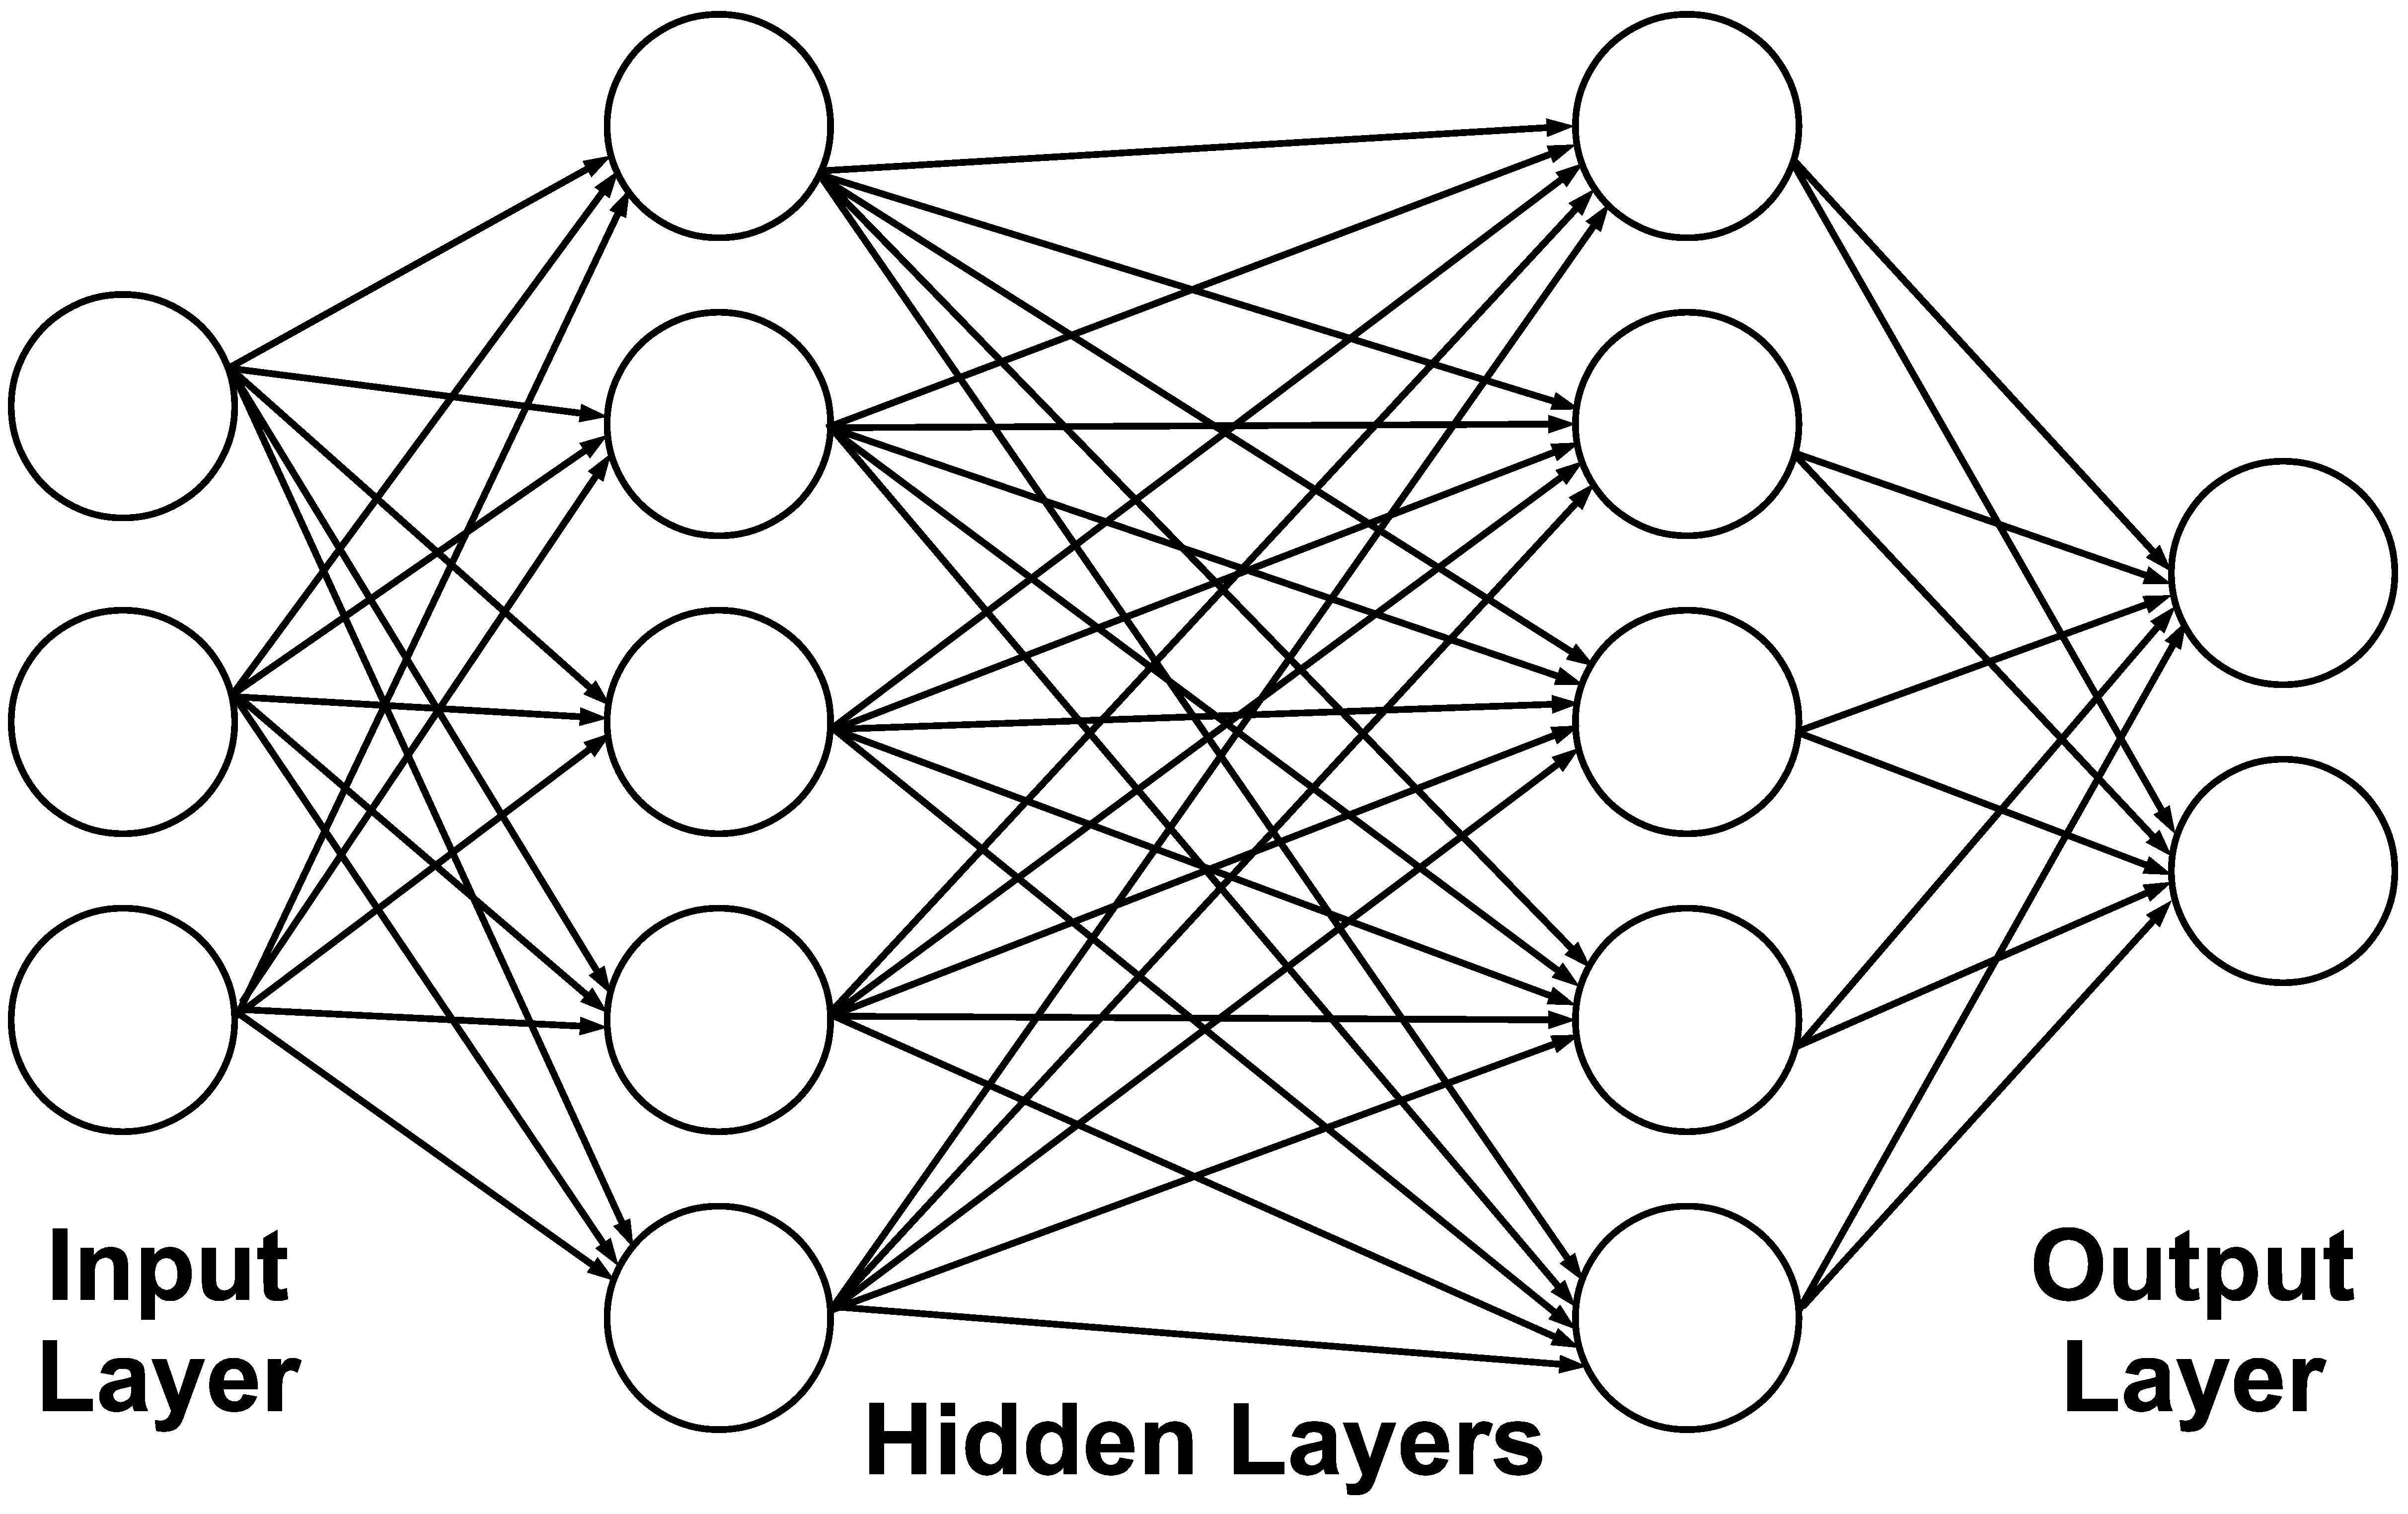
\includegraphics[scale=0.10]{./Images/dnn-diagram.eps}
    \caption{An example of a DNN architecture.}
    \label{dnn_illustration}
\end{figure}

The two units in the output layer (classification layer) represent the genuine and replay speech classes and the
softmax activation function is used in that layer. The posteriors obtained at the output layer of DNN is transformed
into LLR score as
\begin{equation}
    LLR_\mathrm{DNN} = \log p(genuine | \mathbf{X}) - \log p(replay | \mathbf{X})
\end{equation}

In addition, early-stopping algorithm is used during DNN training to achieve best model. The trained model is
validated with a certain frequency using the development data. Then, the model is identified as the best model as soon
as the validation score is found to be better than the previous one. The training and validation process is terminated
when the validation score does not change (early stopping).

\section{Experimental Setup}
\label{experimental_setup}
\subsection{Corpus}
\label{sec:corpus}

ASVspoof 2017 database \cite{kinnunen2017reddots} is used in the experiments. It consists of genuine and replayed
speech signals sampled at 16 kHz and recorded at 16-bit resolution. The database is divided into three non-overlapping
sets: training, development and evaluation. The  statistics (number of speakers, genuine and replay utterances) for
each set is summarized in the Table~\ref{database}.

\begin{table}[ph]
    \centering
    \caption{\textsc{ASVspoof 2017 Database \cite{kinnunen2017reddots}}}
    \vspace{2mm}
    \label{database}
    \begin{tabular}{|c|c|cc|}
        \hline
        Subset      & Speakers & \multicolumn{2}{|c|}{Utterances}          \\
                    &          & Genuine                          & Replay \\
        \hline
        Training    & 10       & 1507                             & 1507   \\
        Development & 8        & 760                              & 950    \\
        Evaluation  & 24       & 1,298                            & 12,008 \\
        \hline
    \end{tabular}
\end{table}

The training set is used to train the spoofing detector. In other words, it is used to train the acoustic models (GMMs
or DNN in this work) for genuine and spoof classes. The development set is used for optimizing the hyper-parameters and
fine tuning the system. Finally the evaluation set contains both genuine and replay spoof speech and is used to test
the actual performance of the system. Although the evaluation set contains speech signals originated from the same
replay configurations as in the training and development sets, the majority of the signals generated using different
configurations. Therefore evaluation set contains replay spoof signals which is unknown (or unseen) for the spoofing
detector. This will reflect the generalization capability of the developed systems. More detailed information about the
database can be obtained from the study \cite{kinnunen2017reddots}. An updated version of the database which includes
fixed versions of some recording environment labels on development and evaluation protocol files was recently released
and details can be found in \cite{delgado2018asvspoof}.

\subsection{Features}
\label{features}
% CQCC
Constant Q cepstral coefficients (CQCC) are the reference features used in this work as previously mentioned. 18
dimensional static CQCC ($c_1 - c_{19}$) features are extracted from the speech signals. The number of features were
optimized after the preliminary experiments conducted on development set of the ASVspoof 2017 database with GMM
classifiers.

% LTAS
\begin{figure}[!htb]
    \centering
    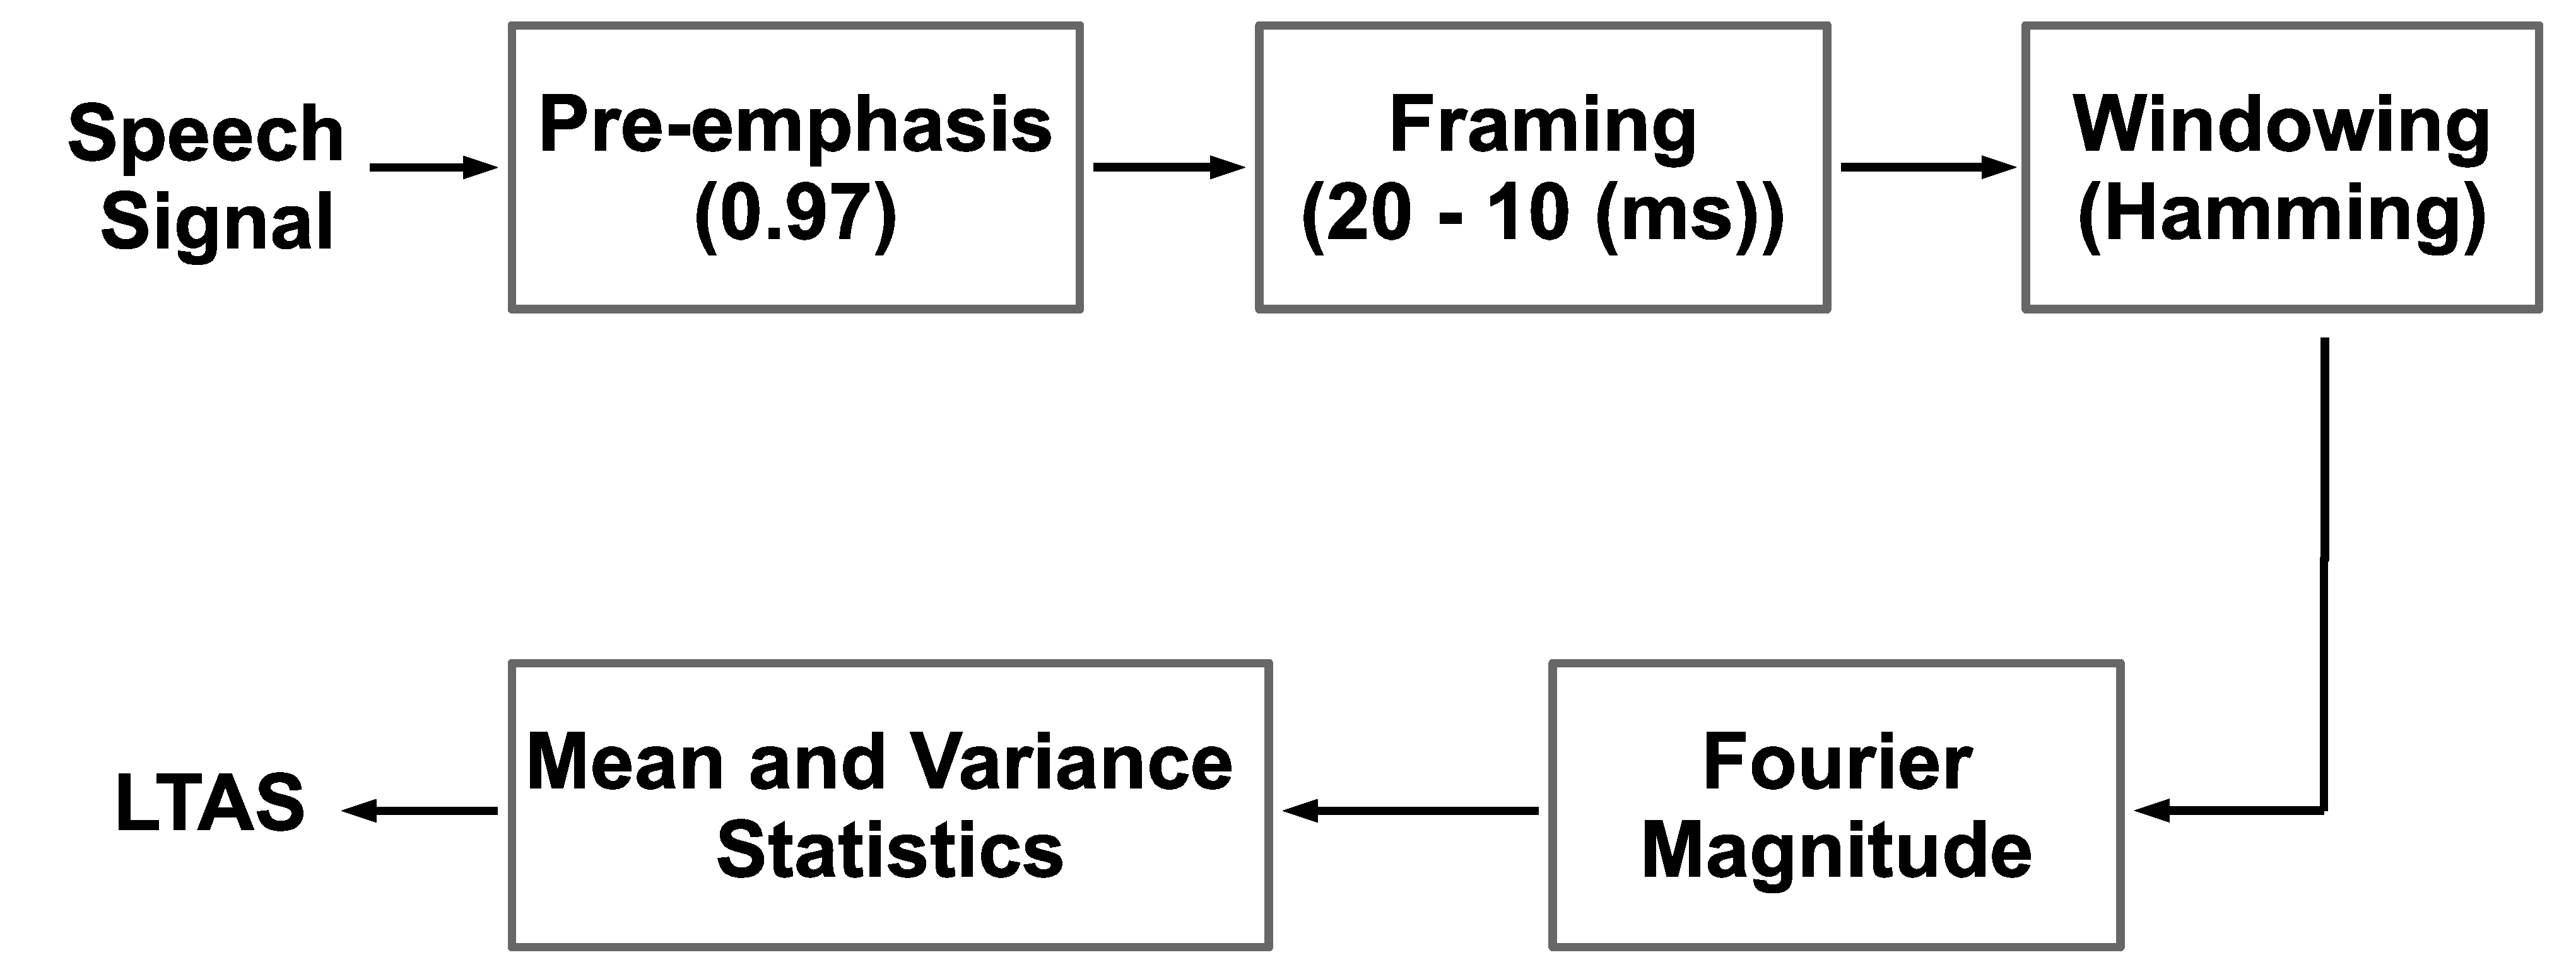
\includegraphics[scale=0.124]{./Images/ltas-diagram.eps}
    \caption{LTAS Feature Extraction Diagram.}
    \label{ltas_diagram}
\end{figure}

Apart from the CQCC, standard mel-frequency cepstral coefficients (MFCC) features \cite{davis1980comparison} are
utilized in the experiments. In MFCC feature extraction, the pre-emphasized speech signal is first divided into 20 ms
frames in every 10 ms. Each frame is multiplied with Hamming window function. The DFT power spectrum of the windowed
frames are calculated using fast Fourier transform (FFT). The power spectrum is then processed by a 27-channel
Mel-filterbank. Discrete cosine transform (DCT) is applied to the logarithmic filterbank outputs which results the MFCC
features.

The third and the last feature type is the long-term average spectrum (LTAS) \cite{muckenhirn2016presentation}. Unlike
the CQCC and MFCC features, LTAS features represents an utterance in a long-term fashion rather than short-term. In
order to extract LTAS features, pre-emphasized speech signal is first split into frames of 20 ms with 10 ms frame
shift. The 512 point DFT of Hamming windowed speech frames is computed using Fast Fourier transform (FFT) to obtain the
logarithmic magnitude spectrum of each frame. The mean and standard deviation of the log-magnitude spectrum is computed
over all frames and these two statistics are concatenated to obtain the final 514 dimensional LTAS feature vector. A
diagram of LTAS feature extraction process is given in Fig. ~\ref{ltas_diagram}.

\subsection{Classifiers}
\label{classifiers}
% GMM
For GMM based replay attack detection system, each class (genuine and replay classes) is represented by a GMM
consisting of 512 components which is trained using 10 EM iterations using the training features of each class.

% DNN
DNN parameters depend on the behavior of the features so the hyper parameters (number of hidden layers, number of
units in each hidden layer, dropout values etc.) vary for each feature type. Although there are some methods to
pre-determine these values, best solution is optimizing them empirically since these values highly depend on data
(features). The DNN configuration for each feature set is optimized using the preliminary experiments are summarized
in Table~\ref{dnn_classfier}.

\begin{table}[!htb]
    \centering
    \caption{\textsc{DNN configuration for each feature set.}}
    \vspace{4mm}
    \label{dnn_classfier}
    \begin{tabular}{|c|c|c|c|}
        \hline
                              & CQCC & MFCC & LTAS \\ \hline
        Input Size            & 18   & 57   & 514  \\
        \# Hidden Layers      & 3    & 3    & 5    \\
        \# Hidden Layer Units & 256  & 256  & 1024 \\
        Dropout Value         & 0.2  & 0.2  & 0.5  \\
        \hline
    \end{tabular}
\end{table}

Batch normalization and dropout placed after every layer. Rectified linear unit (ReLU) is used as the activation
function in every layer except for output layer which is recently the most popular one for deep learning problems.
The softmax activation function is used at the output layer since it is a classification task. The learning rate is
selected as 0.01 and stochastic gradient descent (SGD) optimizer is used for training.

\subsection{Performance Criterion}
\label{performance_criterion}
The equal error rate (EER) is used as the performance metric for replay attack detection in ASVspoof 2017 challenge
\cite{kinnunen2017asvspoof}. EER corresponds to the error rate at the threshold where false acceptance rate (FAR) and
false rejection rate (FRR) are equal. The lower the EER value, the higher the accuracy of the spoofing detection
system. Besides EER, detection error trade-off (DET) curves \cite{martin1997det} are also given to view the overall
performance of the spoofing detection system.

\section{Experimental results}
\label{sec:experimental_work}
\subsection{Results on Development Set}
We first analyzed the effect of sub-band frequency selection which were previously shown to be effective for replay
attack detection on different types of features. We compare the EERs obtained with baseline, MFCC-GMM and LTAS-DNN
systems on development set of the ASVspoof 2017 database by varying the lowest frequency in the range $0\leq f \leq
    8$ kHz in Fig.~\ref{eer_vs_fmin}. More precisely, the lowest frequency used in the feature extraction is varied in
that range. For CQCC, sub-band analysis is performed by applying a high-pass filter (a $4$th order Butterworth filter)
to the speech signal with cut-off frequency corresponding to the low sub-band frequency, whereas for MFCCs it is
performed by placing the mel-filters within the specific frequency range. For LTAS in turn, it was accomplished by
limiting the number of DFT bins. First, LTAS-DNN system outperforms the baseline (CQCC-GMM and MFCC-GMM) systems for
all values of the lowest frequency. Similar to previous observations reported by different studies, it can be seen that
extracting features from a sub-band rather than $0-8$ kHz band, considerably reduces the EER independent of the
features or classifiers. For the baseline and MFCC-GMM systems, 6-8 kHz sub-band was found to yield the lowest EER
(EERs of 8.18\% and 5.54\%, respectively). However, for LTAS-DNN system, extracting the LTAS feature vectors from the
4-8 kHz sub-band shows the best performance with the EER of 4.10\%. The CQCC and MFCC features extracted from the 6-8
kHz sub-band and LTAS features extracted from the 4-8 kHz frequency band will be used throughout the paper.

\begin{figure}[!t]
    \centering
    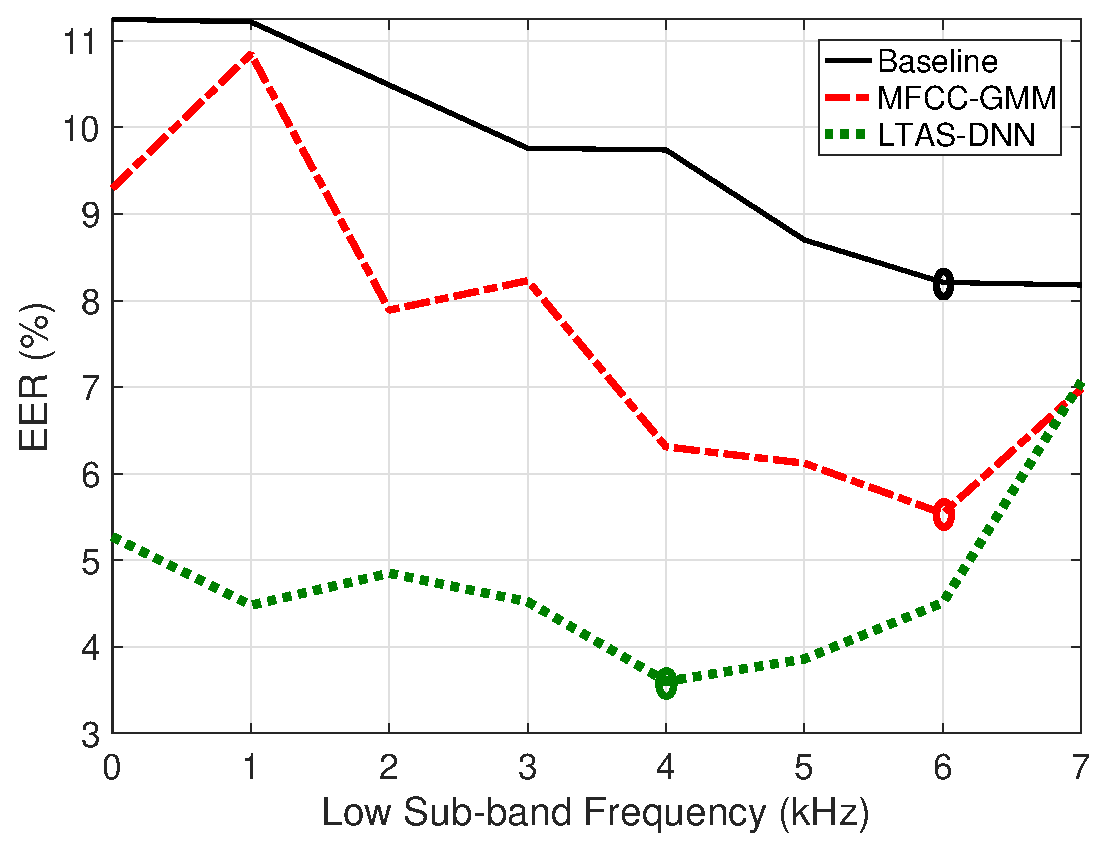
\includegraphics[scale=0.4]{./Images/eer-vs-fmin.eps}
    \caption{Effect of low sub-band frequency on replay attack detection performance for different features.}
    \label{eer_vs_fmin}
\end{figure}

Next, we compare the performances of the GMM and DNN classifiers for replay attack detection on development set in
Table~\ref{dev_res}. One would argue that, the results of LTAS features with GMM classifier is missing in the Table.
GMM technique is suitable for modeling the set of feature vectors whereas LTAS features correspond to a single 514
dimensional feature vector per utterance. From the results reported in Table~\ref{dev_res}, it can be observed that
standard MFCC-GMM system yields approximately 48\% lower EER in comparison to baseline CQCC-GMM (EERs of 5.54\% vs.
8.18\%). The performance gap between CQCC and MFCC features further increases when DNN classifier is utilized although
DNN is inferior to GMM classifier. The results in table show that our DNN approach achieves the smallest EER on
development set.

\begin{table}[!htb]
    \centering
    \caption{\textsc{EERs (\%) on development set.}}
    \vspace{4mm}
    \label{dev_res}
    \begin{tabular}{|c|c|c|}
        \hline
        System     & EER[\%]       \\ \hline
        CQCC - GMM & 8.18          \\
        MFCC - GMM & 5.54          \\
        CQCC - DNN & 10.05         \\
        MFCC - DNN & 6.44          \\
        LTAS - DNN & \textbf{4.10} \\
        \hline
    \end{tabular}
\end{table}

From the results reported in Table~\ref{dev_res} and Fig.~\ref{eer_vs_fmin} it can be seen that short-term features
(MFCC and CQCC) are inferior to LTAS based features independent of the classifier. This is possibly because of the
fact that short-term features convey discriminatory information about not only genuine and replayed signals but also
speaker identity, language and phonetic structure embedded in the signal which are irrelevant for spoofing attack
detection. However, with LTAS approach the effect of these irrelevant features (irrelevant for spoofing detection) are
reduced by computing the average and standard deviation over the frames.

In the last set of experiments on development set, we explore the effect of cepstral zero-mean and unit-variance
normalization (CMVN) on replay attack detection. Applying CMVN to the features does not bring any improvement on the
performance irrespective of the classifier and features. Indeed, it increases the EER considerably. For example the
EER of best performing system (LTAS-DNN) increases from 4.10\% to 6.05\%.

\begin{table}[!htb]
    \centering
    \caption{\textsc{Effect of cmvn on development set.}}
    \vspace{4mm}
    \label{norm}
    \begin{tabular}{|c|c|c|}
        \hline
        System                         & EER[\%]       \\ \hline
        CQCC\textsubscript{CMVN} - GMM & 15.15         \\
        MFCC\textsubscript{CMVN} - GMM & 13.40         \\
        CQCC\textsubscript{CMVN} - DNN & 17.18         \\
        MFCC\textsubscript{CMVN} - DNN & 12.51         \\
        LTAS\textsubscript{CMVN} - DNN & \textbf{6.05} \\
        \hline
    \end{tabular}
\end{table}

\begin{figure}[!t]
    \centering
    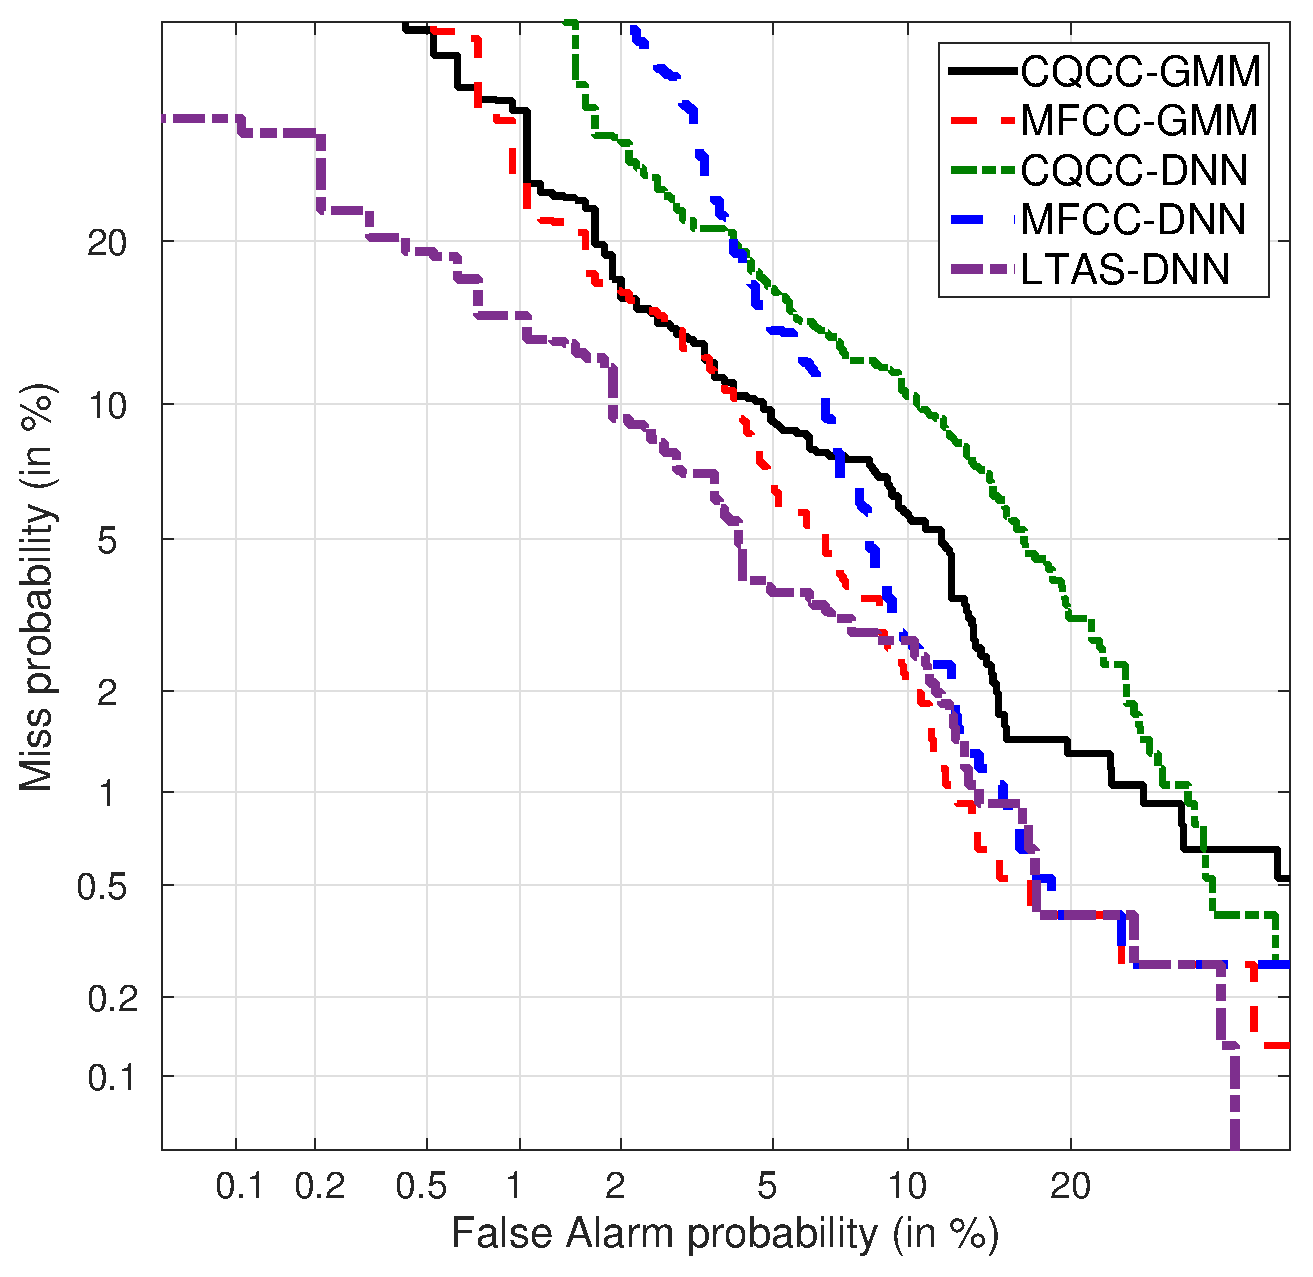
\includegraphics[scale=0.3]{./Images/development-det-curves.eps}
    \caption{DET Curves for Development Set.}
    \label{dev_det}
\end{figure}

Det curves of development set for each system are shown in Fig.~\ref{dev_det}. From the DET curves, LTAS-DNN gives
consistently better performance than other systems for all operating points. However, MFCC-GMM and CQCC-GMM systems
the behaviour of the systems differ for different operating point. For example at the EER point MFCC outperforms CQCC
features whereas at the low False alarm rates, they show similar performance. However, at the high false alarm rates,
the performance gap further increases. Similar observations hold for MFCC-DNN and CQCC-DNN systems.

\subsection{Results on Evaluation Set}
In the evaluation set experiments, we use the features without applying any feature normalization since it was found
to reduce the spoofing attack detection performance considerably on the development set experiments (Table~\ref{norm}).
The results obtained on evaluation set is summarized in Table~\ref{eval_res}. Similar to results on development set,
LTAS-DNN system yields the best performance among the others. However, the EERs are considerably high in comparison to
that of development set. This is because the majority of the replayed speech signals in evaluation set are originated
from different replay configurations than training and development sets. Therefore, these configurations are unknown
to the system.

\begin{table}[h]
    \centering
    \caption{\textsc{EERs (\%) on evaluation set.}}
    \vspace{2mm}
    \label{eval_res}
    \begin{tabular}{|c|c|c|}
        \hline
        System     & EER[\%]        \\ \hline
        CQCC - GMM & 29.94          \\
        MFCC - GMM & 27.74          \\
        CQCC - DNN & 32.64          \\
        MFCC - DNN & 25.34          \\
        LTAS - DNN & \textbf{20.77} \\
        \hline
    \end{tabular}
\end{table}

The LTAS-DNN system yields approximately 44\% lower EER than the baseline system (CQCC-GMM) on evaluation set. The
performance difference between LTAS-DNN and CQCC-DNN systems is even larger (EERs of 20.77\% vs. 32.64\%). For MFCC
features, DNN classifier slightly reduces the EER in comparison to GMM classifier. However, for CQCC features, GMM
classifier is superior to DNN back-end.

Finally, DET curve of each replay attack detection system generated on evaluation set is shown in Fig.~\ref{eval_det}.
Similar to development set (Fig.~\ref{dev_det}), LTAS-DNN is absolute winner at all operating points but with a larger
performance difference than development set. In contrast to development set curves, the curves of other systems are
well separated and they show consistent performance.

\section{Conclusions}
\label{sec:conc}
In this paper, we experimentally investigated the performance of DNN approach for replay attack spoofing detection.
Different than majority of the existing studies which utilize DNN for feature extraction, we employed DNN for
classification purpose. Our experiments show that the long-term average spectrum based features yield better
performance than the CQCC and MFCC features. Best EER values of 4.10\% and 20.77\% were obtained using LTAS features
with DNN classifier for development and evaluation datasets, respectively. It was also found that high frequency range
convey more discriminative information independent from feature and classifier. The feature normalization (CMVN) was
found to increase the EER irrespective of the feature type and classifier.

\begin{figure}[!t]
    \centering
    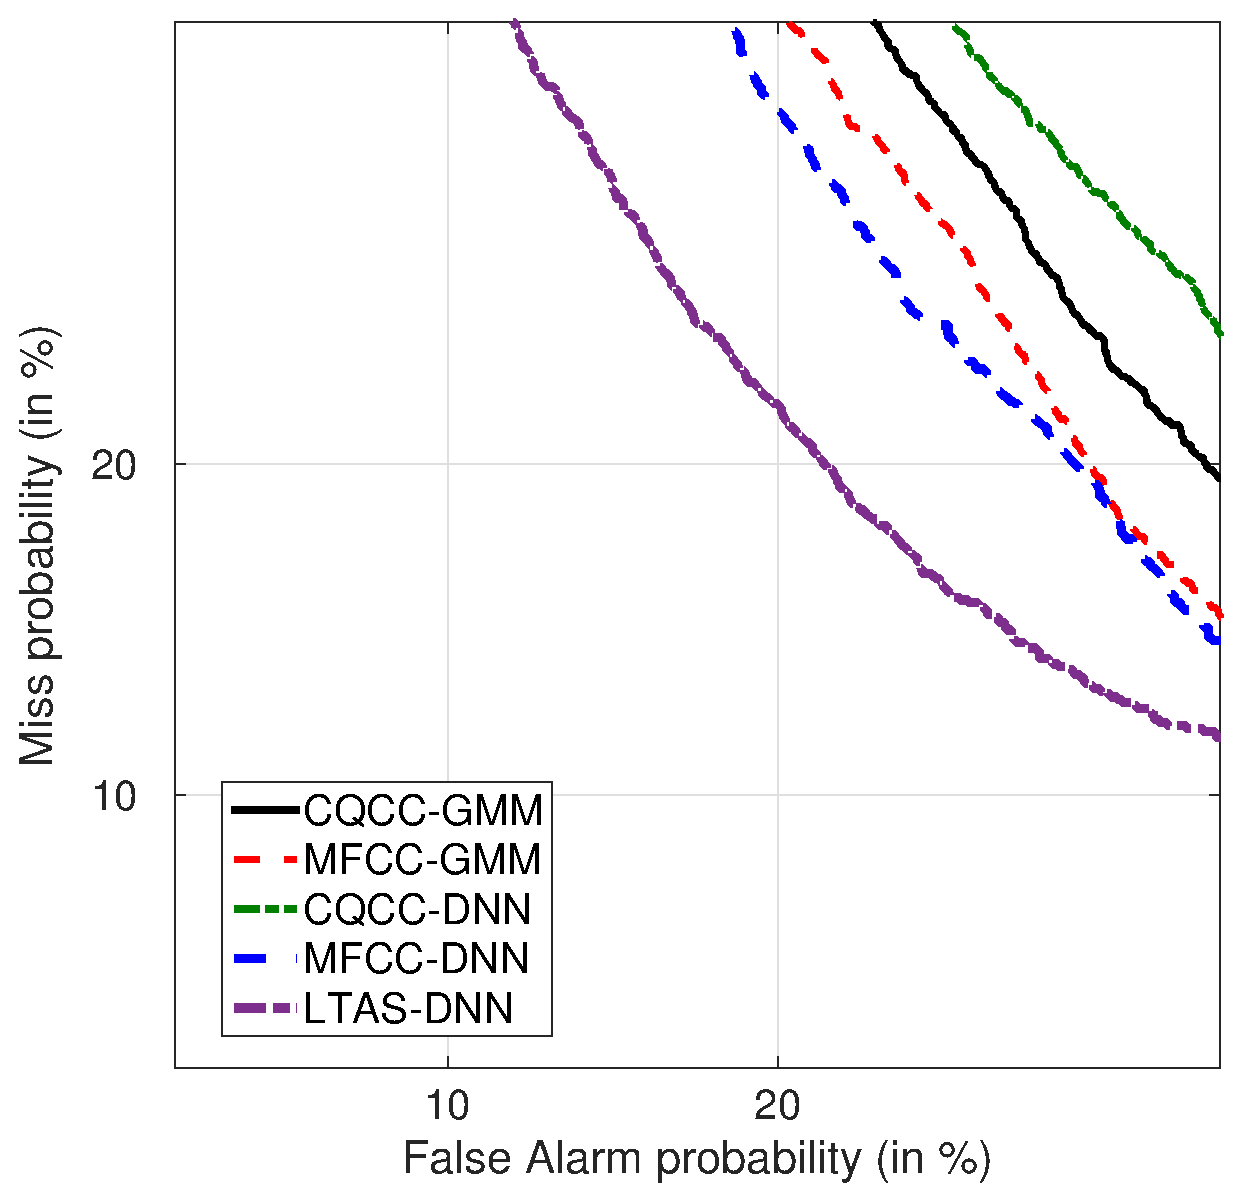
\includegraphics[scale=0.35]{./Images/eval-dets.eps}
    \caption{DET Curves for Evaluation Set.}
    \label{eval_det}
\end{figure}

\bibliographystyle{IEEEbib}
\bibliography{strings, bibliography}

\end{document}
